\documentclass{beamer}
\usepackage[czech]{babel}
\usepackage[utf8]{inputenc}
\usetheme{Pittsburgh}
\title{Vytváření dopředné neuronové sítě pomocí algoritmu Tiling}
\institute{FIT VUT v Brně}
\author{Jan Sedlák}
\date{2013}
\begin{document}

\begin{frame}
  \maketitle
\end{frame}

\begin{frame}{Algoritmus Tiling}
  Dynamické vytváření neuronové sítě:
  \begin{itemize}
    \item klasifikace pouze do dvou skupin,
    \item používá perceptrony,
    \item pro učení pocket algoritmus,
    \item v každé vrstvě musí dosáhnout ``věrohodnosti''.
  \end{itemize}
\end{frame}

\begin{frame}{Princip fungování}
\begin{columns}
  \begin{column}{0.47\textwidth}
    \begin{itemize}
    \item První neuron je Master:
      \begin{itemize}
      \item snaží se co nejlépe klasifikovat vstup,
      \item algoritmus končí vytvořením posledního Master neuronu.
      \end{itemize}
    \item Další neurony ve vrstvě jsou Ancillary:
      \begin{itemize}
      \item snaží se zaručit věrohodnost vrstvy.
      \end{itemize}
    \end{itemize}
  \end{column}
  \begin{column}{0.5\textwidth}
    \includegraphics{nn.eps}
  \end{column}
\end{columns}
\end{frame}

\begin{frame}{}
\end{frame}

\begin{frame}{}
\end{frame}

\begin{frame}{}
\end{frame}

\end{document}
